% This is "sig-alternate.tex" V1.9 April 2009
% This file should be compiled with V2.4 of "sig-alternate.cls" April 2009
%
% This example file demonstrates the use of the 'sig-alternate.cls'
% V2.4 LaTeX2e document class file. It is for those submitting
% articles to ACM Conference Proceedings WHO DO NOT WISH TO
% STRICTLY ADHERE TO THE SIGS (PUBS-BOARD-ENDORSED) STYLE.
% The 'sig-alternate.cls' file will produce a similar-looking,
% albeit, 'tighter' paper resulting in, invariably, fewer pages.
%
% ----------------------------------------------------------------------------------------------------------------
% This .tex file (and associated .cls V2.4) produces:
%       1) The Permission Statement
%       2) The Conference (location) Info information
%       3) The Copyright Line with ACM data
%       4) NO page numbers
%
% as against the acm_proc_article-sp.cls file which
% DOES NOT produce 1) thru' 3) above.
%
% Using 'sig-alternate.cls' you have control, however, from within
% the source .tex file, over both the CopyrightYear
% (defaulted to 200X) and the ACM Copyright Data
% (defaulted to X-XXXXX-XX-X/XX/XX).
% e.g.
% \CopyrightYear{2007} will cause 2007 to appear in the copyright line.
% \crdata{0-12345-67-8/90/12} will cause 0-12345-67-8/90/12 to appear in the copyright line.
%
% ---------------------------------------------------------------------------------------------------------------
% This .tex source is an example which *does* use
% the .bib file (from which the .bbl file % is produced).
% REMEMBER HOWEVER: After having produced the .bbl file,
% and prior to final submission, you *NEED* to 'insert'
% your .bbl file into your source .tex file so as to provide
% ONE 'self-contained' source file.
%
% ================= IF YOU HAVE QUESTIONS =======================
% Questions regarding the SIGS styles, SIGS policies and
% procedures, Conferences etc. should be sent to
% Adrienne Griscti (griscti@acm.org)
%
% Technical questions _only_ to
% Gerald Murray (murray@hq.acm.org)
% ===============================================================
%
% For tracking purposes - this is V1.9 - April 2009

\documentclass{Group6_Phase2}

\begin{document}
%
% --- Author Metadata here ---
%\conferenceinfo{WOODSTOCK}{'97 El Paso, Texas USA}
%\CopyrightYear{2007} % Allows default copyright year (20XX) to be over-ridden - IF NEED BE.
%\crdata{0-12345-67-8/90/01}  % Allows default copyright data (0-89791-88-6/97/05) to be over-ridden - IF NEED BE.
% --- End of Author Metadata ---

\title{Group 6 - Phase 1}
%\subtitle{[Extended Abstract]}
%
% You need the command \numberofauthors to handle the 'placement
% and alignment' of the authors beneath the title.
%
% For aesthetic reasons, we recommend 'three authors at a time'
% i.e. three 'name/affiliation blocks' be placed beneath the title.
%
% NOTE: You are NOT restricted in how many 'rows' of
% "name/affiliations" may appear. We just ask that you restrict
% the number of 'columns' to three.
%
% Because of the available 'opening page real-estate'
% we ask you to refrain from putting more than six authors
% (two rows with three columns) beneath the article title.
% More than six makes the first-page appear very cluttered indeed.
%
% Use the \alignauthor commands to handle the names
% and affiliations for an 'aesthetic maximum' of six authors.
% Add names, affiliations, addresses for
% the seventh etc. author(s) as the argument for the
% \additionalauthors command.
% These 'additional authors' will be output/set for you
% without further effort on your part as the last section in
% the body of your article BEFORE References or any Appendices.

\numberofauthors{2} %  in this sample file, there are a *total*
% of EIGHT authors. SIX appear on the 'first-page' (for formatting
% reasons) and the remaining two appear in the \additionalauthors section.
%
\author{
% You can go ahead and credit any number of authors here,
% e.g. one 'row of three' or two rows (consisting of one row of three
% and a second row of one, two or three).
%
% The command \alignauthor (no curly braces needed) should
% precede each author name, affiliation/snail-mail address and
% e-mail address. Additionally, tag each line of
% affiliation/address with \affaddr, and tag the
% e-mail address with \email.
%
%	1st. author
	\alignauthor
		Kevin Dombrosky\\
		       \affaddr{Rochester Institute of Technology Student}\\
		       \affaddr{610 Park Point Dr}\\
		       \affaddr{Rochester, New York 14623}\\
		       \email{kfd6490@rit.edu}
%	2nd. author
	\alignauthor
		Brittany Purcell\\
		       \affaddr{Rochester Institute of Technology Student}\\
		       \affaddr{107 Weldon Street}\\
		       \affaddr{Rochester, New York 14611}\\
		       \email{blp6903@rit.edu}
}

\maketitle
\begin{abstract}
This paper discusses the progression of the group project for Group 6 in the Intro to Big Data class at Rochester Institute of Technology, CSCI-620. The paper will further explain the work that has been done so far, what will be done in the future, and what the expectations are for the finished project. 
\end{abstract}

\keywords{Phase 2, Group 6, Plants}

\section{Introduction}
The group project for CSCI-620, Intro to Big Data at Rochester Institute of Technology has been underway for 9 weeks now. Is has been about about 2 weeks since the last phase update, and since then a lot of work has gone into the database and visualization. 

As a recap there are two requirements for the project. The first is a database management system (DBMS), which for this project will be a relational database system in MSQL which contains a dataset from the UCI Machine Learning Repository(http://archive.ics.uci.edu/ml/datasets/Plants).\\* The second requirement is the visualization, which is an application that shows the geographical location of various types of plants in the United States and Canada. The information for the visualization will be contained in that dataset from the UCI website. 

There has been steady progression toward this goal, and so far there have been no changes to the visualization design, or the dataset. 
\\\\\\\\\\\\\\

\section{Body}

\subsection{Database}
As a reminder, the dataset is be set up in a MySQL database. In order to move the data from the .txt files into the dataset, a script was written. Originally the script was going to be written in Python, however Java was chosen later due to its familiarity with the group. The script needed to break down the files in an easy to read way so the MySQL Workbench could be used to load the data into the tables. Below is, first the ER-diagram which represents how the database will interact, the second is the original file contents that need to be interpreted to work in the database. 

\begin{figure}[htb]
	\centering
	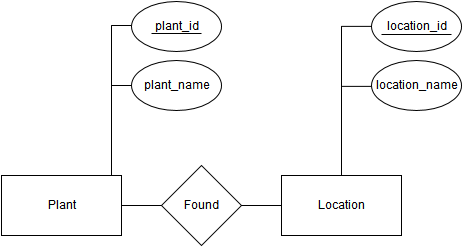
\includegraphics[scale=0.5]{FinalProject_ERdiagram.png}
	\caption{The ER diagram which represents the organization of the data in the database.}
\end{figure}

\begin{figure}[htb]
	\centering
	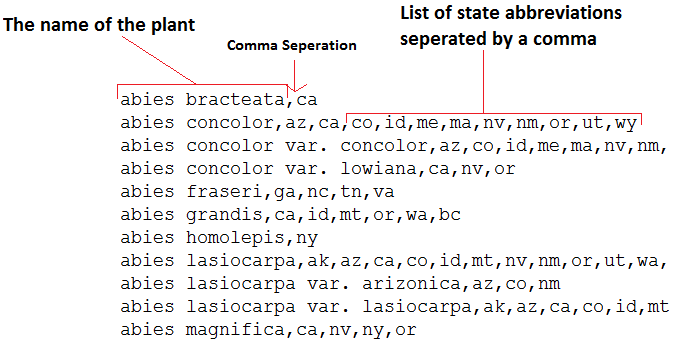
\includegraphics[scale=0.4]{original_database_file.png}
	\caption{The organization of the original database file.}
\end{figure}

As a reminder, for the database there were going to be three tables, each with two columns. 
\begin{description}
	\item[Table Layouts:] \hfill
	\begin{itemize}
		\item Plant Table
			\begin{itemize}
				\item IDplant
				\item plantname
			\end{itemize}
		\item State Table
		\begin{itemize}
			\item IDstate
			\item statename
		\end{itemize}
		\item PlanttoState Table
		\begin{itemize}
			\item IDplant
			\item IDstate
		\end{itemize}
	\end{itemize}
\end{description}

In order for MySQL to load the information into the tables, the .txt files need to be converted so that the files contained the information in the order that it would appear in the columns, separated by a tab character. So, for example in the Plant table, the plant\_data.txt file would need to contain an ID, tab character, plant name. This is the same for each of the tables that need to be loaded. If the .txt files are in the correct order it is a simple LOAD call in MySQL to load the tables. 


\begin{description}
	\item[Steps to Database Loading:] \hfill
	\begin{enumerate}
		\item Creating a text file for the plant data that contains the plant name and plant id. The plant ID was just generated, starting at 1, and going until there were no more plants in the original file (which a snippet of can be seen in the figure above). The name then, was just the first element in every line of the file. Each line in the file was a different plant, so each would have a unique ID.
		\item Next, the states needed to be organized into the state table, which also contained an ID and a name. The dataset provided the following file, which contained the states and their abbreviations that are used. (http://archive.ics.uci.edu/ml \\* /machine-learning-databases/plants/stateabbr.txt) This, for now, was used to access the full names of the locations, since that is what will be used by the visualization. Again, the ID's were created based on the amount of locations that were read in, and the state names were the second item in every line, only this time separated by a space and not a comma. 
		\item The last part was the trickiest. Since the PlanttoState table is looking only at the ID's of the states and plants, those needed to first be determined for each plant, and added into a text file. For this the original file (seen again in Figure 2) has the abbreviations for the states. The script kept track of the abbreviation to name connection for states, and the name to ID connection. So, in order to find the state ID associated with a specific abbreviation there had to be a lookup. The plant ID was simple, since the name and ID were connected, but the state lookup was a little more in depth. In the end, there was a text file that contained a plant ID and a state ID, each line representing either another state the plant was found in, or the next plant on the list. (This is so that in the PlanttoState table there are only the two columns)
		\item Once all three of the text files were created, the following LOAD call needed to be made to load the information. This call will be made three times (one for each table that needed to be loaded). \\* \\* LOAD DATA LOCAL INFILE 'filelocation' INTO TABLE tablename COLUMNS TERMINATED BY '\t'; \\*
	\end{enumerate}
\end{description}


\subsection{Application}
Group 6 decided to create a visualization for this class, which was discussed in Phase-0. As a recap, the visualization will consist of a map(functional for only the United States and Canada), as well as a search box for the user to search for a certain plant. This has been created, and the screen shot of the application is in Figure 2 below. 

This application is a web page that will be written in Jade Markup Language with CSS. This is the language that is most familiar to the group, after one of the members worked with the language all summer on an independent project. The basic blueprint for the web page has already been created(again, see Figure 2), but it has not yet been hooked up to the database. 

Ultimately, there will be (on the left hand side of the website right below the search bar) a list of plants that are found in the database. The user can search for a specific plant (using the search bar) which will highlight the regions that plant is located. Otherwise, the user can choose a plant from the list, and it will do the same thing. Another option for users would be to select a region they are interested in, and the list on the left would change to be only plants that can be found in that area. 

\begin{figure}[htb]
	\centering
	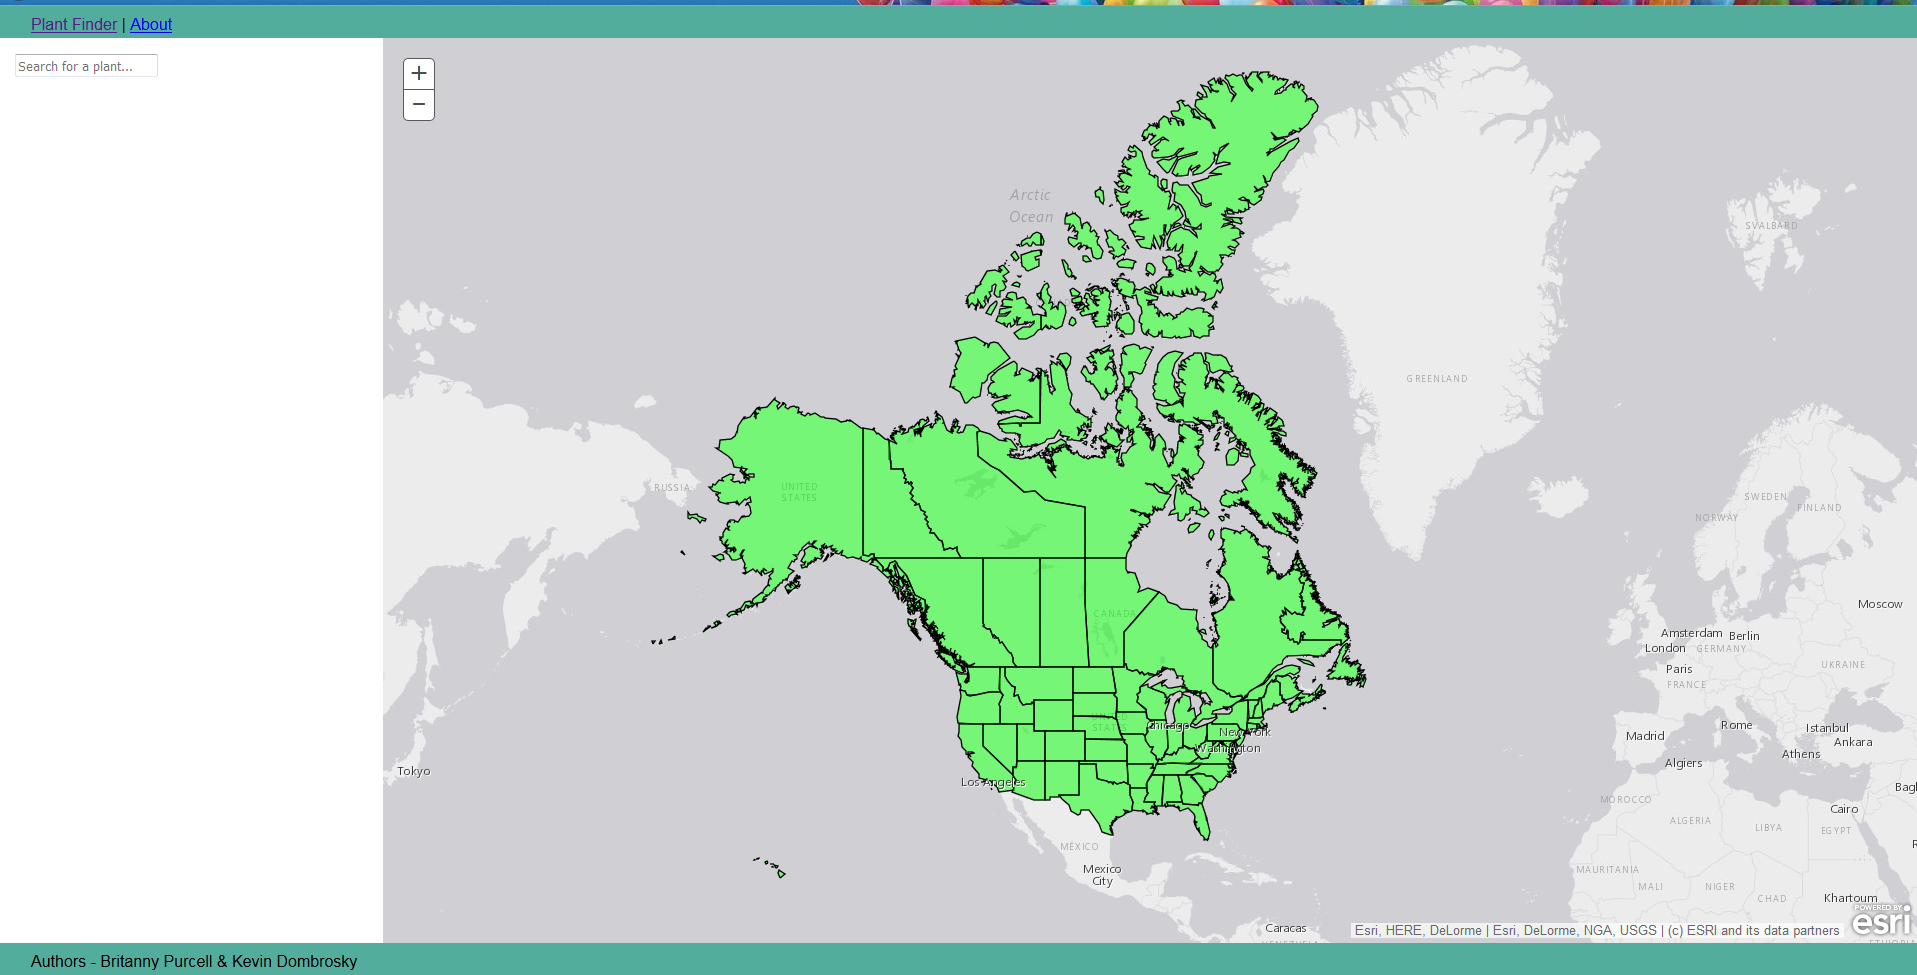
\includegraphics[scale=0.17]{Website_Screenshot.png}
	\caption{A screen shot of the website being used for the application.}
\end{figure}
\subsection{Communication}
In order for the website and database to communicate, the database will be setup on a Node.js server. This will allow the website to request information from the local database, which is set up using MySQL Server. In order for the user interface(UI) to change based on users requests, this is how the information will be transmitted from the database to the website. 

\subsection{Data Analyses}
The data analyses will all happen through the website visualization. A user will be able to either select a state or a plant in order to find information from the database. If a state is selected, then, on the left hand side of the website, a list of plants that can be found in this location will appear, and all the other states will be changed to the color white. The other option is using the search bar to find a plant. This will actually use substring searching, so as you are searching a list of possible plants will appear, and all the locations occupied by these plants that match the substring will be highlighted. This works the same for searching a specific plant name. The locations in which the plant can be located will become highlighted on the screen in green. This is a simple way to take the information found in the data set and portray it in an easy to read and easy to see way for any user. Now, a user can find a list of plants that grow in their location, or find out if a plant in a specific location can be found.

\subsection{Resources}
There are many different resources being used in order to develop the project. These include certain files, softwares, and online databases all assisting in the creation of the website and database. As it was already covered, the database is being set up as a MySQL database running on a local server set up using MySQL Server, the application will be a website visualization that is coded using Jade and CSS, and the database and website will communicate with a Node.js server. 

The code is being stored using GitHub, and is shared among all members of the group. This is a repository to store, download, and change the existing code. The code is being written in different platforms, some members are using Notepad++ to do the coding, while others are using Visual Studio Code. The scripts to load the database were written in Eclipse, using Java coding language. Once the code is written in each of these mediums, the code is added to the GitHub repository. 

LaTeX is being used to write the ACM style templates, which is the document you are currently reading, and Visual Studio Code is used for the README(which will walk users through how to run the program and access the website).

The README will be provided to establish step-by-step instructions on downloading and installing necessary software, and (once the software is installed), how to run the project and access the website. There is also README's on how to get the data set information in the .txt files into a local database using MySQL Workbench. 


\section{Conclusions}
The group has already made some progress towards finishing the project. This includes work on both the application as well as the database. There is still much work that needs to be done, but most of the thinking and setting up has been finished. Languages and applications have been chosen and are in the process of being set up. Below is a quick list of what was done, what needs to be done, and deliverables that have been set.  

\begin{description}
	\item[Accomplished:] \hfill
	\begin{itemize}
		\item Developed ER Diagram
		\item Created Website Wire Frame
		\item Setup Website
		\item Conceptualized Application Utilization
		\item Wrote a Java Script to change dataset text files
		\item Loaded the dataset into MySQL database
		\item Set up the database on a local server using MySQL Server
	\end{itemize}
	
	\item[To Be Done:] \hfill
	\begin{itemize}
		\item Establish Communication Between Website and Database
		\item Display Information on Website
		\item Change Display Based on User Input
	\end{itemize}
	
	\item[Resources] \hfill
	\begin{itemize}
		\item GitHub
		\item LaTeX
		\item Node.js
		\item Notepad++
		\item Visual Studio Code
		\item Eclipse
		\item MySQL WorkBench
		\item MySQL Server
		\item Java
	\end{itemize}
	
	\item[Files] \hfill
	\begin{itemize}
		\item README
		\item Group6-Phase2
		\item CSCI620-master (Folder)
		\item plant\_data.txt
		\item state\_data.txt
		\item plant\_to\_state\_data.txt
	\end{itemize}
\end{description}


\section{Citations}
\begin{itemize}
	\item Relevant Papers
	\begin{itemize}	
		\item H\"{a}m\"{a}l\"{a}inen, W. and Nyk\"{a}nen, M.: Efficient discovery of statistically significant association rules. Proceedings of the 8th IEEE International Conference on Data Mining (ICDM 2008), pp. 203-212. IEEE Computer Society 2008. 			
	\end{itemize}		
	\item Dataset
		\begin{itemize}		
			\item USDA, NRCS. 2008. The PLANTS Database ([Web Link], 31 December 2008). National Plant Data Center, Baton Rouge, LA 70874-4490 USA.
		\end{itemize}	
\end{itemize}


\end{document}  % This is where a 'short' article might terminate
